\begin{titlepage} % Suppresses displaying the page number on the title page and the subsequent page counts as page 1
	\newcommand{\HRule}{\rule{\linewidth}{0.5mm}} % Defines a new command for horizontal lines, change thickness here
	
	\center % Centre everything on the page
	
	%------------------------------------------------
	%	Headings
	%------------------------------------------------
	
	\textsc{\LARGE IT University of Copenhagen}\\[1.5cm] % Main heading such as the name of your university/college
	
	\textsc{\Large Computer Science Master Thesis, MSc}\\[0.5cm] % Major heading such as course name

    \textsc{\large STADS - KISPECI1SE}\\[0.5cm]

    \textsc{\large Examination Group - S25KISPECI1SE767}\\[0.5cm]
 
	
	%------------------------------------------------
	%	Title
	%------------------------------------------------

    \vfill
    
	{\huge\bfseries Python Application Energy Consumption:\\ Investigating Operating System, Python Version and Hardware Impact on the Energy Consumption of Application Benchmarks}\\[1cm] % Title of your document
	
    \vfill


	%------------------------------------------------
	%	Author(s)
	%------------------------------------------------
    \AddToShipoutPictureBG*{%
      \AtPageLowerLeft{%
        \transparent{0.4}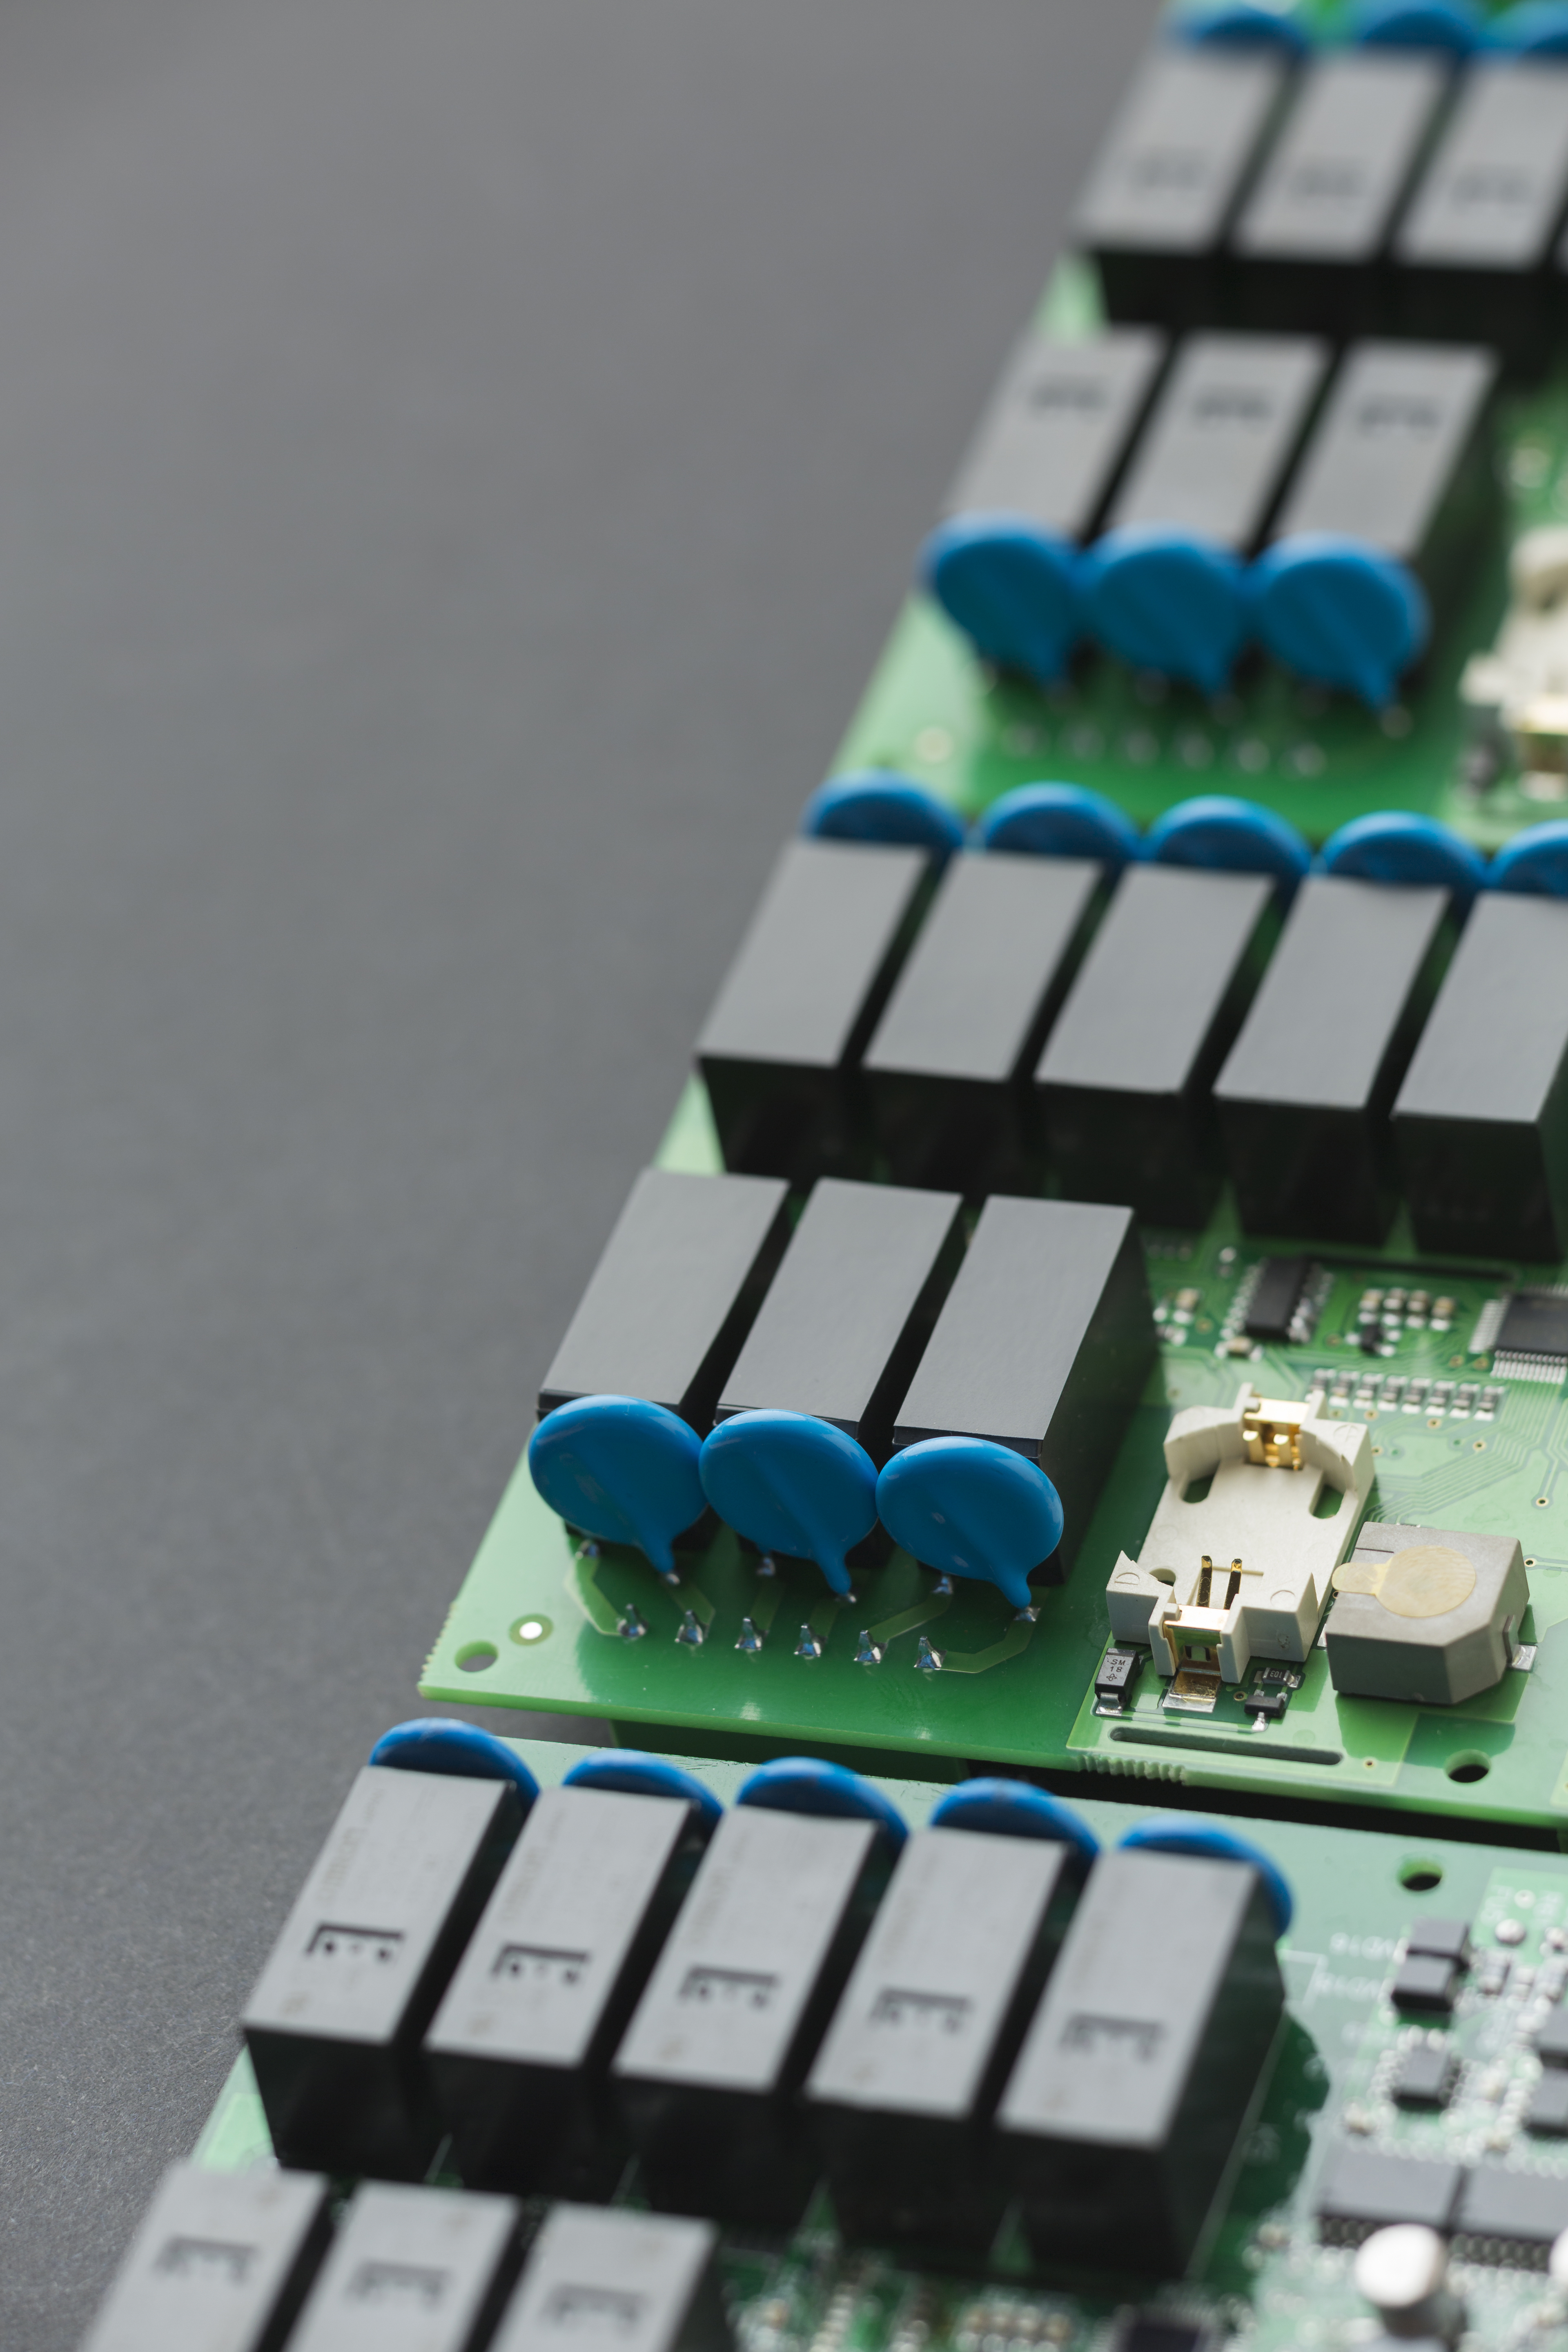
\includegraphics[width=\paperwidth,height=\paperheight]{pictures/frontpage.jpg}%
      }%
    }
	
	\begin{minipage}{0.4\textwidth}
		\begin{flushleft}
			\large
			\underline{\textit{Student:}}\\
            \textbf{Oskar Emil Breindahl}\\    \textit{osbr@itu.dk} \\
		\end{flushleft}
	\end{minipage}
	~
	\begin{minipage}{0.4\textwidth}
		\begin{flushright}
			\large
			\underline{\textit{Supervisor:}}\\
			\textbf{Helge Pfeiffer} % Supervisor's name
			\\
			\textit{ropf@itu.dk}
			\\
		\end{flushright}
	\end{minipage}
	
	% If you don't want a supervisor, uncomment the two lines below and comment the code above
	%{\large\textit{Author}}\\
	%John \textsc{Smith} % Your name
	
	%------------------------------------------------
	%	Date
	%------------------------------------------------
	
	\vfill
	
	%{\large\bfseries The Figma Prototype can be Found at }\\[0.4cm]
	%\href{https://www.figma.com/file/Xep84e2FRmQlw55MkzaZii/Wireframes?node-id=22\%3A3}{https://www.figma.com/file/Xep84e2FRmQlw55MkzaZii/Wireframes?node-id=22\%3A3}
	
	\vfill\vfill\vfill % Position the date 3/4 down the remaining page
	
	\begin{center}
	    \
	    June 2, 2025
	\end{center} % Date, change the \today to a set date if you want to be precise
	
	%------------------------------------------------
	%	Logo
	%------------------------------------------------
	
	%\vfill\vfill
	%\includegraphics[width=0.2\textwidth]{placeholder.jpg}\\[1cm] % Include a department/university logo - this will require the graphicx package
	 
	%----------------------------------------------------------------------------------------
	
	\vfill % Push the date up 1/4 of the remaining page
	
\end{titlepage}